\documentclass[]{article}

\usepackage{hyperref}
\usepackage{graphicx}
\usepackage{mathtools}
\usepackage{amssymb}
%\usepackage{enumitem}
\usepackage{paralist}
\usepackage{csquotes}
\usepackage[affil-it]{authblk}
\usepackage{listings}
\usepackage{tikz}
\usetikzlibrary{shapes,arrows,decorations.pathreplacing,calc}

\begin{document}

\pagestyle{headings}  % switches on printing of running heads

\title{Machine Learning Methods in Functional Programming and Interactive Theorem Proving}

\author{Chris Warburton}

\affil{University of Dundee,\\
\texttt{http://tocai.computing.dundee.ac.uk}}

\maketitle              % typeset the title of the contribution

\begin{abstract}
Since their inception, computers have been applied to automate and assist work in mathematics, with established fields including numerical computation, computer algebra, (online) communication and so on. Here we focus on their use in two areas: formal proof and statistics; and how new approaches are bringing these seemingly disparate disciplines closer together.
\end{abstract}

\section{Introduction}

As computers and software become more capable, and as our reliance on them increases, the importance of \emph{understanding}, \emph{predicting} and \emph{verifying} these systems grows; which is undermined by their ever-increasing complexity. Mathematics provides us with powerful, systematic methods of reasoning, which we can bring to bear on this challenge; in particular those of \emph{formal logic} and \emph{statistics}. By (partially) mechanising these approaches, in the fields of \emph{theorem proving} and \emph{machine learning}, respectively, we can leverage these increasing machine capabilities and direct them for the purpose of analysis. However, the question still remains: on what should we focus that analysis?

In this work, we investigate the notion of \emph{interestingness} in the exploration of formal systems (an area known as \emph{theory exploration}) as a way to make productive use of resources in an often intractable domain. To keep things concrete, we focus our formal analysis on equational formulae describing programs in the Haskell language, for reasons elaborated in \S \ref{haskell}. Conceptually, we maintain a broader view, and survey many related areas which may offer insights on the problem.

Appeals to interestingness arise when more direct measures, such as utility, are not available. For example, the inclusion of particular statements in a program or proof development can be easily justified based on its contribution to the overall solution; however, in a \emph{library} there is no particular problem being solved, in which case we must judge statements on less direct criteria, such as how ``interesting'' they may be to our users. Appeals to interestingness abound in the history of computer-assisted reasoning; for example, in 1971 Plotkin \cite{plotkin1971further} considered the task of \textquote{discovering theorems $T$ from a system of axioms $Ax$}, and in particular the questions \textquote{Under what conditions is $T$ an interesting, possible theorem in the system $Ax$?} and \textquote{Is there a way to generate (most) interesting possible theorems?}. Despite such widespread use of the term, there is no standard definition of what makes a formal object, whether it is an axiom, a conjecture, a proof, etc., ``interesting''; although many ad-hoc heuristics have been proposed.

We begin our undertaking in \S \ref{background} by introducing the Haskell language, as well as the relevant fields of verification for context. We define a formal framework for our investigation, and show how it relates to the existing theorem proving landscape. A selection of theorem proving scenarios which \emph{require} exploration are discussed in \S \ref{examples}, whilst related work, including existing defintions of interestingness, is surveyed in \S \ref{relatedwork}. We also review the use of exploration in other fields of Artificial Intelligence and Machine Learning, where researchers are also experimenting with replacing \emph{explicit} goals and rewards with \emph{implicit} alternatives such as interestingness. Recent efforts in this area have lead to principled theories to emerge, mostly based around (algorithmic) information theory, which may be adapted to our theory exploration context.

We discuss our present contributions in \S \ref{current} and future research directions in \S \ref{future}, before concluding in \S \ref{conclusion}.

\section{Background}
\label{background}

Most work in mechanised, formal mathematics focuses on a \emph{theorem proving} paradigm, usually either \emph{interactive theorem proving} (ITP) or \emph{automated theorem proving} (ATP). Whilst the boundaries between these approaches can be somewhat blurred, we give precise definitions in \S \ref{itp} and \S \ref{atp}, respectively, and characterise both as being \emph{goal-driven}: particular conjectures must be provided as input to the process, and the output is either a proof, a refutation or ``don't know'' (in the case of incomplete procedures).

In this work, we instead adopt the paradigm of \emph{(automated) theory exploration}, discussed in \S \ref{theoryexploration}, which includes the ability to \emph{generate} conjectures, and hence output \emph{novel} theorems. Since many theories will admit an infinite number of trivial theorems (e.g. $\top$, $\top \land \top$, $(\top \land \top) \land \top$, \dots) we require some mechanism for avoiding such undesirable, yet provable, statements. This is the role of interestingness, which we can use to \emph{judge} a statement, in a potentially rich way, rather than merely constructing or failing to construct a proof.

Firstly, however, we give an overview of the Haskell programming language in \S \ref{haskell}. This allows us to establish many concepts in a straightforward software context, which we can then re-use in the potentially less-familiar realm of interactive theorem proving. We decided to focus on Haskell, as it has mature, state-of-the-art theory exploration implementations (\textsc{QuickSpec} \cite{QuickSpec} and \textsc{HipSpec} \cite{claessen2013automating}). This is evident even to users of Isabelle/HOL, which boasts its own \textsc{IsaCoSy} \cite{johansson2009isacosy} and \textsc{Hipster} \cite{Hipster} theory exploration systems, since \textsc{Hipster} is actually implemented by translating to Haskell and invoking \textsc{HipSpec}.

\subsection{Haskell}\label{haskell}

\lstset{
  frame=none,
  xleftmargin=2pt,
  stepnumber=1,
  numbers=none,
  numbersep=5pt,
  numberstyle=\ttfamily\tiny\color[gray]{0.3},
  belowcaptionskip=\bigskipamount,
  captionpos=b,
  escapeinside={*'}{'*},
  language=haskell,
  tabsize=2,
  emphstyle={\bf},
  commentstyle=\it,
  stringstyle=\mdseries\rmfamily,
  showspaces=false,
  keywordstyle=\bfseries\rmfamily,
  columns=flexible,
  basicstyle=\small\sffamily,
  showstringspaces=false,
  morecomment=[l]\%,
}

\providecommand{\hs}[1]{\lstinline[language=Haskell]|#1|}

Haskell is a programming language which is well-suited to research; indeed, this was a goal of the language's creators \cite{marlow2010haskell}. Like most members of the \emph{functional programming} paradigm, Haskell is essentially a variant of $\lambda$-calculus; in fact the \textsc{GHC} compiler uses (variants of) the polymorphic $\lambda$-calculus \emph{System F} as an intermediate representation (referred to a \emph{GHC Core}). For a detailed exposition of the language syntax and semantics, you can consult the Haskell Language Report \cite{marlow2010haskell} \footnote{Version 2010 was current as this was written}; here we will focus on those language features which make it particularly suited for our formal reasoning purposes:

\begin{description}

\item{Functional}: All control flow is performed by function abstraction and application, which we can reason about using standard rules of inference such as \emph{modus ponens}.

\item{Pure}: Execution of actions (e.g. reading files) is separate to evaluation of expressions; hence our reasoning can safely ignore complicated external and non-local interactions.

\item{Statically Typed}: Expression are constrained by \emph{types}, which can be used to eliminate unwanted combinations of values, and hence reduce search spaces; \emph{static} types can be deduced syntactically, without having to execute the code.

\item{Non-strict}: If an evaluation strategy exists for $\beta$-normalising an expression (i.e. performing function calls) without diverging, then a non-strict evaluation strategy will not diverge when evaluating that expression. This is rather technical, but in simple terms it allows us to reason effectively about a Turing-complete language, where evaluation may not terminate. For example, when reasoning about \emph{pairs} of values \hs{(x, y)} and projection functions \hs{fst} and \hs{snd}, we might want to use an ``obvious'' rule such as $\forall \text{\hs{x y}}, \text{\hs{x}} = \text{\hs{fst (x, y)}}$. Haskell's non-strict semantics makes this equation valid; whilst it would \emph{not} be valid in the strict setting common to most other languages, where the expression \hs{fst (x, y)} will diverge if \hs{y} diverges (and hence alter the semantics, if \hs{x} doesn't diverge).

\item{Algebraic Data Types}: These provide a rich grammar for building up user-defined data representations, and an inverse mechanism to inspect these data by \emph{pattern-matching}. For our purposes, the useful consequences of ADTs and pattern-matching include their amenability for inductive proofs and the fact they are \emph{closed}; i.e. an ADT's declaration specifies all of the normal forms for that type. This makes exhaustive case analysis trivial, which would be impossible for \emph{open} types (for example, consider classes in an object oriented language, where new subclasses can be introduced at any time).

\item{Parametricity}: This allows Haskell \emph{values} to be parameterised over \emph{type-level} objects; provided those objects are never inspected. This has the \emph{practical} benefit of enabling \emph{polymorphism}: for example, we can write a polymorphic identity function \hs{id :: forall t. t -> t}. \footnote{Read ``\hs{a :: b}'' as ``\hs{a} has type \hs{b}'' and ``\hs{a -> b}'' as ``the type of functions from \hs{a} to \hs{b}''.} Conceptually, this function takes \emph{two} parameters: a type \hs{t} \emph{and} a value of type \hs{t}; yet only the latter is available in the function body, e.g. \hs{id x = x}. This inability to inspect type-level arguments gives us the \emph{theoretical} benefit of being able to characterise the behaviour of polymorphic functions from their type alone, a technique known as \emph{theorems for free} \cite{wadler1989theorems}.

\item{Type classes}: Along with their various extensions, type classes are interfaces which specify a set of operations over a type (or other type-level object, such as a \emph{type constructor}). Many type classes also specify a set of \emph{laws} which their operations should obey but, lacking a simple mechanism to enforce this, laws are usually considered as documentation. As a simple example, we can define a type class \hs{Semigroup} with the following operation and associativity law:

\begin{lstlisting}[language=Haskell, xleftmargin=.2\textwidth, xrightmargin=.2\textwidth]
op :: forall t. Semigroup t => t -> t -> t
\end{lstlisting}

$$\forall \text{\hs{x y z}}, \text{\hs{op x (op y z)}} = \text{\hs{op (op x y) z}}$$

The notation \hs{Semigroup t =>} is a \emph{type class constraint}, which restricts the possible types \hs{t} to only those which implement \hs{Semigroup}. \footnote{Alternatively, we can consider \hs{Semigroup t} as the type of ``implementations of \hs{Semigroup} for \hs{t}'', in which case \hs{=>} has a similar role to \hs{->} and we can consider \hs{op} to take \emph{four} parameters: a type \hs{t}, an implementation of \hs{Semigroup t} and two values of type \hs{t}. As with parameteric polymorphism, this extra \hs{Semigroup t} parameter is not available at the value level. Even if it were, we could not alter our behaviour by inspecting it, since Haskell only allows types to implement each type class in at most one way, so there would be no information to branch on.} There are many \emph{instances} of \hs{Semigroup} (types which may be substituted for \hs{t}), e.g. \hs{Integer} with \hs{op} performing addition. Many more examples can be found in the \emph{typeclassopedia} \cite{yorgey2009typeclassopedia}. This ability to constrain types, and the existence of laws, helps us reason about code generically, rather than repeating the same arguments for each particular pair of \hs{t} and \hs{op}.

\item{Equational}: Haskell uses equations at the value level, for definitions; at the type level, for coercions; at the documentation level, for typeclass laws; and at the compiler level, for ad-hoc rewrite rules. This provides us with many \emph{sources} of equations, as well as many possible \emph{uses} for any equations we might discover. Along with their support in existing tools such as SMT solvers, this makes equational conjectures a natural target for our investigation.

\end{description}

Together, these features make Haskell code highly structured, amenable to logical analysis and subject to many algebraic laws. However, as mentioned with regards to type classes, Haskell itself is incapable of expressing or enforcing these laws (at least, without difficulty \cite{lindley2014hasochism}). This reduces the incentive to manually discover, state and prove theorems about Haskell code, e.g. in the style of interactive theorem proving (see \S \ref{itp}), as these results may be invalidated by seemingly innocuous code changes. We will revisit the second-class status of theorem proving in Haskell in our discussion of theory exploration (\S \ref{theoryexploration}), but we will remark that Haskell in thus in a unique position with regards to the discovery of interesting theorems. Namely that many discoveries may be available with very little work, simply because the code's authors are focused on \emph{software} development rather than \emph{proof} development. The same cannot be said, for example, of ITP systems; although our reasoning capabilities may be stronger in an ITP setting, much of the ``low hanging fruit'' will have already been found through the user's dedicated efforts, and hence TE would be more likely to fit into an automation role for the user, rather than providing truly unexpected new discoveries.

Other empirical advantages to studying Haskell, compared to either other programming languages or theorem proving systems, include:

\begin{itemize}

\item The large amount of Haskell code which is freely available online, e.g. in repositories like \href{http://hackage.haskell.org}{Hackage}, with which we can experiment.

\item The existence of conjecture generation and theory exploration systems for Haskell, such as \textsc{QuickSpec} and \textsc{HipSpec}, and counterexample finders like \textsc{QuickCheck}, \textsc{SmallCheck} and \textsc{SmartCheck}.

\item The remarkable amount of infrastructure which exists for working with Haskell code, including package managers, compilers, interpreters, parsers, static analysers, etc.

\end{itemize}

\subsection{Interactive Theorem Proving}
\label{itp}

ITP is based around a \emph{proof checker} $C$, which is a decision procedure for determining if a given value $P$ (known as a \emph{proof object} or \emph{witness}) consititutes a proof of a given statement $S$:

$$ C \colon (P \times S) \rightarrow Boolean $$

The process of ITP can hence be understood as the search for an appropriate $P$ for our \emph{goal} $S$:

$$ ITP \colon (S \times C) \rightarrow \{ P \mid C(P, S) = True \} $$

It just so happens that a useful way to implement such a system is via pure functional programming, with the result that many ITP systems (AKA \emph{proof assistants}) such as Coq and Agda appear very similar to languages like Haskell. In particular, we can represent statements $S$ as types and proofs $P$ as values, in which case the proof checker $C$ is simply a type-checker. There are some obvious quirks, such as the need to be \emph{total} (not Turing-complete) in order to ensure soundness, but overall many of the features we introduced for Haskell, such as parametricity, type classes and ADTs are directly translatable to the ITP setting.

This coincidence is due to the \emph{Curry-Howard correspondence} \cite{wadler2015propositions}, which identifies programming languages with systems of logic. Functional programming languages correspond to intuitionistic logics, and are hence a natural fit for reasoning on computers. With additional axioms, we can extend these to more familiar classical logics, although these can make it harder to compute.

Most differences between functional programming and ITP stem from different \emph{expectations} of the user. In the case of Haskell, the desire for expressivity outweighs the desire for soundness, and hence its designers opted to make it Turing-complete. For an ITP language like Agda, soundness far outweighs the inconvenience of having to prove termination, so the opposite tradeoff is made. Similarly, since many ITP ``programs'' (proofs) will never be executed, the language can avoid optimisation in favour of simplicity (and hopefully correctness). This approach is summed up by the \emph{de Bruijn criterion}, which requires that the system \textquote{generates 'proof-objects' (of some form) that can be checked by an 'easy' algorithm} \cite[\S~2]{barendregt2001proof} \cite{barendregt2001proof}. One nice consequence of this approach, which is followed for example by Isabelle \cite{nipkow2002isabelle} and Coq \cite{bertot2013interactive}, is that the proof assistants themselves can become arbitrarily complex and even buggy, yet as long as the proof checker remains simple we can maintain a high degree of our confidence in the results.

Their emphasis on \emph{interactivity}, mostly caused by operating in undecidable domains, means ITP can require an enormous effort for non-trivial proof or verification tasks (e.g. see \cite{hales2015formal}). One common way to mitigate this problem is by implementing powerful \emph{tactics}: meta-programs which automate as much of a proof as possible. The most striking example of such meta-programming is the \emph{Sledgehammer} component of Isabelle/HOL \cite{journals/iandc/MengQP06}, which invokes a multitude of ATP systems on (a translated form of) the current goal to see if any can provide a proof which Isabelle's core checker will accept.

\subsection{Automated Theorem Proving}
\label{atp}

ATP systems are similar in principle to proof assistants, but are based around a \emph{proof search} algorithm rather than a proof checker. By using a fixed algorithm for proving, such as \emph{resolution} \cite[\S~9.6]{Russell:2003:AIM:773294} or \emph{superposition} \cite{bachmair1994rewrite}, ATP programs are limited to particular decidable or semi-decidable fragments of logic. In particular, most ATP systems (such as E \cite{schulz2013system} and Vampire \cite{riazanov2003implementing}) operate in classical first-order logic. This is the most striking difference from ITP systems (e.g. Coq, Agda and Isabelle) which operate in higher-order logics.

In addition to its interest to logicians, ATP has been actively researched in the field of artificial intelligence, dating back to the founding of the field at the 1956 Dartmouth conference. Even by that time Newell and Simon has developed their Logic Theory Machine \cite{newell1956logic}, which was subsequently able to prove theorems like those in Principia Mathematica \cite{newell1958elements}. The approaches now known as \emph{good old-fashioned AI} (GOFAI) were due in part to the success of automated theorem proving, as attempts were made to formulate many problems in a form amenable to first-order reasoning.

Recently there has been a trend away from this direction, towards statistical formulations amenable to machine learning, which we will review in \S \ref{related}.

\subsection{Theory Exploration}
\label{theoryexploration}

The most striking difference between theory exploration (TE) and theorem proving is the former's lack of an explicit goal (e.g. a user-provided conjecture to prove). Instead, the \emph{implicit} goal is more open-ended: the discovery of ``interesting'' conclusions from the given premises. Of course, a key question to ask is what do we mean by ``interesting''? There is no single answer, although many approximate measures have been proposed. The choice of what counts as ``interesting'' has been used to classify various TE implementations \cite{warburtonscaling}, along with their approaches to term generation, well-formedness and proof.

Following \cite{warburtonscaling}, we call a pair $(\Sigma, V)$, of a signature and a set of variables, a \emph{theory}. \emph{Theory exploration} then refers to any process $(\Sigma, V) \overset{TE}{\rightarrow} \text{Terms}(\Sigma, V)$ for producing terms of the theory which are well-formed, provable and ``interesting''.

The conditions of well-formedness and provability can be handled through the use of type systems and automated theorem provers. Hence the method of conjecture generation, and the determination of what is interesting, are the most important properties of any TE system.

Early implementations like \textsc{Theorema} \cite{buchberger2000theory} provided interactive environments, similar to computer algebra systems and interactive theorem provers, to assist the user in finding theorems. Like in the ITP approach, the relatively simple process of verification is automated, whilst the more difficult tasks (term generation and the determination of their interest) are left up to the user.

Subsequent systems have investigated \emph{automated} theory exploration, for tasks such as lemma discovery \cite{Hipster}. By removing user interaction, these properties must be implemented by algorithms. In existing systems these are tightly coupled to improve efficiency, which makes it difficult to try different approaches independently.

As an example, \textsc{QuickSpec} \cite{QuickSpec} discovers equations about Haskell code, which are defined as ``interesting'' if they cannot be simplified using previously discovered equations. The intuition for such criteria is to avoid special cases of known theorems, such as $0 + 0 = 0$, $0 + 1 = 1$, etc. when we already know $0 + x = x$. Whilst this interestingness judgement is elegantly implemented with a congruence closure relation (version 1) and a term rewriting system
(version 2), the conjecture generation is performed in a brute-force way.

Although \textsc{QuickSpec} only \emph{tests} its equations rather than proving them, it is still used as the exploration component of more rigorous systems like \textsc{HipSpec} and \textsc{Hipster}.

\textsc{HipSpec} is currently the most powerful TE system for Haskell, and also forms a major component of \textsc{Hipster}. It uses off-the-shelf ATP programs (including AltErgo, Vampire, Z3, E, SPASS and CVC4) to verify the conjectures of \textsc{QuickSpec}. \textsc{QuickSpec}, in turn, enumerates all type-correct combinations of the terms in the theory up to some depth, groups them into equivalence classes using the \textsc{QuickCheck} counterexample finder, then conjectures equations relating the members of these classes. This approach works well as a lemma generation system, making \textsc{HipSpec} a capable inductive theorem prover as well as a theory exploration system \cite{claessen2013automating}. \textsc{HipSpec} is also compatible with Haskell's existing testing infrastructure, such that an invocation of \texttt{cabal test} can run \textsc{HipSpec} alongside more traditional QA tools like \textsc{QuickCheck}, \textsc{HUnit} and \textsc{Criterion}.

In fact, there are similarities between the way a TE system like \textsc{HipSpec} can generalise from proving \emph{particular} theorems to \emph{inventing} theorems, and the way counterexample finders like \textsc{QuickCheck} can generalise from testing \emph{particular} expressions to \emph{inventing} expressions to test. There are likely lessons that each can learn from the other's approach to term generation.

% Theory exploration is similar to \emph{experimental mathematics}

% - Relation to Science
%  - Testable/falsifiable hypotheses are like evaluable terms (or, more generally, conjectures which can be decided, using a reasonable amount of resources).
% - Relation to AI tasks: exploring surroundings, etc.

% - Statistics is another area that's less straightforward than normal numerical computing, since there is subjectivity and judgement involved in the answering of questions.

% Theory formation: Alison? Others.
% Theory exploration: Buchberger, Moa in Isabelle, Koen in Haskell. Others?
% Theorem proving: Well-trodden: first-order ATP, higher-order ITP, functional programming
% Communication: Latex, Wikis, APIs, communicating with aliens

\section{Exploration in Theorem Proving}
\label{examples}

Before exploring abstract definitions of interestingness, we can first consider some scenarios which arise during formal proof where we are forced to generate conjectures. An analysis of these situations, and the subsequent theorems they produce, will contribute towards an empirical justification for what is interesting (at least from a utilitarian point of view) and inform our later exploration of the literature.

\subsection{Generalisation}

\providecommand{\coq}[1]{\lstinline[language=ML]|#1|}

When we \emph{generalise} a statement $S$, we obtain a new statement $S'$ of which $S$ is a special case. Although counterintuitive, a generalised statement can sometimes be \emph{easier} to prove than the original. This arises often in inductive proofs, since the specific obligations which arise in the proof may be incompatible with the available inductive hypotheses.

However, we cannot blindly generalise \emph{all} obligations we encounter, since \emph{over-generalising} results in obligations which are so strong that they are unprovable, or even false. We must therefore rely on heuristics to guide the generation of generalised conjectures, and hence perform a kind of exploration.

\subsubsection{Tail-recursion}

A classic example of generalisation occurs when we try to reason about \emph{tail-recursive} definitions \cite{kapur2003automatic}. Consider the following Coq functions, defined for the Peano naturals \coq{Z} and \coq{S}:

\begin{lstlisting}[language=ML, xleftmargin=.2\textwidth, xrightmargin=.2\textwidth]
Inductive Nat : Set := Z : Nat
                     | S : Nat -> Nat.

Fixpoint plus      (n m : Nat) := match n with
                                      | Z    => m
                                      | S n' => S (plus n' m)
                                  end.

Fixpoint plus_tail (n m : Nat) := match n with
                                      | Z    => m
                                      | S n' => plus_tail n' (S m)
                                  end.
\end{lstlisting}

\iffalse
Haskell equivalent:

plus :: Nat -> Nat -> Nat
plus      n  Z    = n
plus      n (S m) = S (plus n m)

plus_tail :: Nat -> Nat -> Nat
plus_tail n  Z    = n
plus_tail n (S m) = plus_tail (S n) m
\fi

Both of these functions implement addition, but the \coq{plus_tail} variant is tail-recursive; i.e. it can be implemented in constant space using a loop. However, if we want to \emph{prove} that the definitions are (pointwise) equal, we run into difficulties:

\begin{lstlisting}[language=ML, xleftmargin=.2\textwidth, xrightmargin=.2\textwidth]
(* Solve equalities by beta-normalising both sides *)
Ltac triv := try (simpl; reflexivity).

(* Prove equivalence of plus and plus_tail *)
Theorem equiv : forall n m, plus n m = plus_tail n m.
  induction n; triv. (* Base case is trivial *)

  (* Inductive case: plus (S n) m = plus_tail (S n) m *)
  intro m.

  (* Beta-reduce the right-hand-side (justification is trivial) *)
  replace (plus_tail (S n) m) with (plus_tail n (S m)); triv.

  (* Use induction hypothesis to replace plus_tail with plus *)
  rewrite <- (IHn (S m)).
\end{lstlisting}

At this point we must prove \coq{plus (S n) m = plus n (S m)}, which seems reasonable. However, if we try to proceed by another induction on \coq{n}, we get stuck with incompatible induction hypotheses. Specifically, the \emph{conclusion} of our new induction hypothesis is exactly the equation we need:

\begin{lstlisting}[language=ML, xleftmargin=.2\textwidth, xrightmargin=.2\textwidth]
IHn' : (forall x, plus n' x = plus_tail n' x) -> plus (S n') m = plus n' (S m)
\end{lstlisting}

Yet we cannot provide it with the argument it needs, as our original induction hypothesis is \emph{too specific} (i.e. it has too many \coq{S} constructors):

\begin{lstlisting}[language=ML, xleftmargin=.2\textwidth, xrightmargin=.2\textwidth]
IHn : forall x, plus (S n') x = plus_tail (S n') x
\end{lstlisting}

We are forced to abandon the proof, despite such a reasonable-looking intermediate goal. In fact, we \emph{can} prove that goal in isolation:

\begin{lstlisting}[language=ML, xleftmargin=.2\textwidth, xrightmargin=.2\textwidth]
Lemma gen n m : plus (S n) m = plus n (S m).
  induction n; triv. (* Base case is trivial *)

  (* Move all S constructors outside *)
  simpl. rewrite <- IHn. simpl.

  (* Trivial *)
  reflexivity.
Defined.
\end{lstlisting}

We can now resume our proof of \coq{equiv}, which is easily discharged:

\begin{lstlisting}[language=ML, xleftmargin=.2\textwidth, xrightmargin=.2\textwidth]
  rewrite (gen n m).
  reflexivity.
Defined.
\end{lstlisting}

\subsubsection{Associativity}

As a concrete example, we can take Boyer and Moore's proof of the associativity of multiplication in ACL2 \cite{boyer1983proof}:

$$(x * y) * z = x * (y * z)$$

During the course of the proof, the following obligation arises:

\begin{equation}
  \tag{conc3}
  (y + (x * y)) * z = (y * z) + ((x * y) * z)
  \label{eq:conc3}
\end{equation}

ACL2 automatically generalises \eqref{eq:conc3} by replacing the repeated sub-term $x * y$ with a fresh variable $w$:

\begin{equation}
  \tag{conc4}
  (y + w) * z = (y * z) + (w * z)
  \label{eq:conc4}
\end{equation}

This generalised form is clearly the distributivity law for multiplication and addition, which can be proved separately to the original goal of associativity. It would not be controversial to claim that this distributivity law is interesting in its own right (relative to associativity, at least), in addition to its usefulness in making this proof go through.

The ACL2 heuristics which lead to this result are described as

\subsection{Intention}

One consideration when generating conjectures is the difference (if any) between theorems, lemmas, corollaries, etc. From a logical point of view, these are all equivalent; it Most proof assistants do not distinguish between these, although some (like Coq) may allow users to annotate their statements with label.

\subsection{QuickCheck Properties}



\section{Related Work}
\label{related}

\subsection{Conjecture Generation}

The task of \emph{conjecture generation} lies at the heart of theory exploration, and

\subsubsection{Lemma generation}

\subsection{Exploration in Artificial Intelligence}

Theorem proving is not the only area of AI to have automation extended from problem \emph{solving} to problem \emph{invention}. Here we consider similar approaches in a variety of domains, and identify techniques which could be re-purposed in the context of theory exploration.

\subsubsection{Evolutionary Computation}

\emph{Evolutionary computation} is an umbrella term for heuristic search algorithms which mimic the process of evolution by natural selection among a population of candidate solutions \cite{back1997evolutionary}. Whilst \emph{genetic algorithms} are perhaps the most well-known instance of evolutionary computation, their use of \emph{strings} to represent solutions causes complications in a domain like theory exploration, where recursive structures of unbounded depth arise. Thankfully these problems are not insurmountable, for example \emph{genetic programming} can operate on tree-structures natively \cite{banzhaf1998genetic}, which makes evolutionary computation a viable approach to the search component of theory exploration.

Traditionally, evolutionary approaches assign solutions a \emph{fitness} value, using a user-supplied \emph{fitness function}. Fitness should correlate with how well a solution solves the user's problem; for example, the fitness of a solution to some engineering problem may depend on the estimated materials cost.

The evolutionary analogue of theory exploration is to remove the (explicit) fitness function, just like we remove explicit goals to turn the theorem proving task into the theory exploration task. There are two main reasons for studying such purely-exploratory evolutionary systems: \emph{artificial life} and \emph{deceptive problems}. The former attempts to gain insight into the nature of life and biology through competition over limited resources. Whilst this may have utility in resource allocation, e.g. efficient scheduling of a portfolio of ATP programs, there is no direct connection to the search aspect of theory exploration, so we will not consider it further (note that similar resource-usage ideas can also be found in the literature on \emph{artificial economies}, e.g. \cite{baum2000evolution}).

On the other hand, work on deceptive problems is highly relevant, as it has lead to studying \emph{exploration in general}, and hence provides insight for our narrower domain of theory exploration. Deceptive problems are those where \textquote{pursuing the objective may prevent the objective from being reached} \cite{lehman2011abandoning}, which is caused by the fitness (objective) function having many local optima which are easy to find (eg. by hill climbing), but few global optima which are hard to find. Many approaches to avoiding deception, such as \emph{niching methods} \cite{sareni1998fitness}, alter the output of the fitness function to promote \emph{diversity} and \emph{novelty}. For example, \emph{fitness sharing} promotes diversity by dividing up the fitness of identical or similar solutions, e.g. the result of a fitness function $f$ may be shared by two identical solutions $s_1$ and $s_2$, such that the augmented fitness $f'(s_1) = \frac{f(s_1)}{2}$ and $f'(s_2) = \frac{f(s_2)}{2}$. As always, there are many variations on this theme, such as how to judge similarity (e.g. ``genetically'' by comparing the solutions themselves, or ``phenotypically'' by comparing their fitness), but all strive to penalise duplication and hence promote diversity.

Once we augment fitness functions, to a greater or lesser degree, an obvious question arises: what if the augmented function contains nothing of the original fitness? This is the pure exploration scenario we are interested in, which has been found to provide useful ``stepping stones'', even in objective-driven domains \cite{lehman2011abandoning}.

% TODO: Expand

\subsubsection{Artificial Curiosity}
\label{curiosity}

\begin{figure}
  \centering
  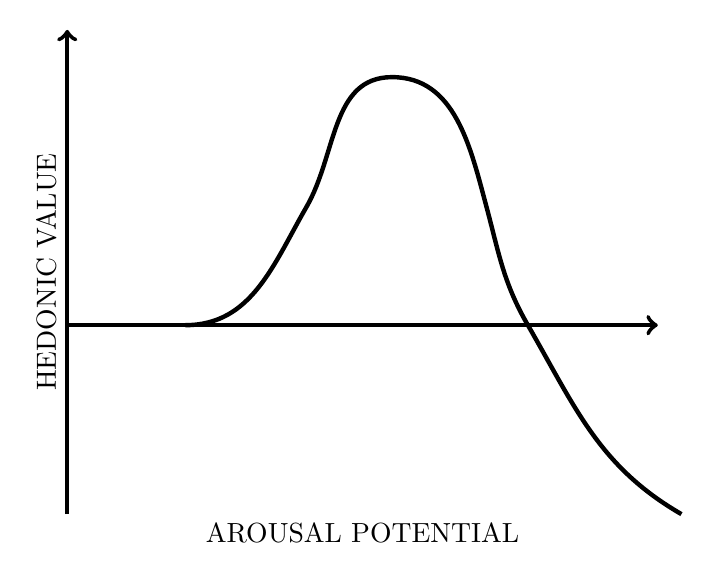
\begin{tikzpicture}[scale=0.75]
      % The image, for reference
      % \node[anchor=south west,inner sep=0] at (0,0) {\includegraphics[width=\textwidth]{wundt.png}};

      % Axes
      \draw[black,ultra thick,->] (1,0.8) -- (1,  9)   node[midway, above, sloped] {HEDONIC VALUE};     % y axis
      \draw[black,ultra thick,->] (1,4)   -- (11, 4);                                                   % x axis
      \path                       (1,0.8) -- (11, 0.8) node[midway, below]         {AROUSAL POTENTIAL}; % x axis label

      % Curve. The numbers come from tracing over wundt.png
      \draw[black,ultra thick] (3, 4)
           to[out=0,   in=240] (5.05, 6)
           to[out=60,  in=180] (6.5,  8.2)
           to[out=0,   in=105] (8.1,  6)
           to[out=-75, in=120] (8.8,  4)
           to[out=-60, in=150] (11.4, 0.8);

      % This version is closer, but a little jagged
      \iffalse
      \draw[black,ultra thick] (3, 4)
           to[out=0,   in=240] (5.05, 6)
           to[out=60,  in=225] (6,    8)
           to[out=45,  in=180] (6.5,  8.2)
           to[out=0,   in=135] (7.2,  8)
           to[out=-45, in=105] (8.1,  6)
           to[out=-75, in=120] (8.8,  4)
           to[out=-60, in=150] (11.4, 0.8);
      \fi
  \end{tikzpicture}

  \caption{The Wundt curve, reproduced from \cite{berlyne1970novelty}. The axes ``hedonic value'' and ``arousal potential'' are described as covering \textquote{reward value\dots preference or pleasure}, and \textquote{all the stimulus properties that tend to raise arousal, including novelty and complexity}, respectively.}

  \label{wundt}
\end{figure}

\emph{Artificial curiosity} (AC) describes learning systems which are rewarded based on the interesting of the input or data they discover \cite{schmidhuber2006developmental}, and hence provides a general mechanism for converting goal-driven algorithms into exploration systems. As an unsupervised learning task, AC has no access to labels or meanings associated with this input; the only features it can learn are the structure and relationships inherent in the data. The aim of AC methods is to force systems away from inputs which are not amenable to learning; either because they are so familiar that there is nothing left to learn, or so unfamiliar that they are unintelligible. The resulting behaviour is characterised by the \emph{Wundt curve} (shown in figure \ref{wundt}) \footnote{(In fact, many measures avoid negative values for simplicity, in which case we can just replace all negative points on the curve with zero.}, which has been used in psychology to explain human aesthetics and preferences \cite{berlyne1970novelty}.

We can divide AC approaches into two groups: the first, which we call \emph{explicit}, send inputs which follow a Wundt curve to their learning algorithm; the second, the \emph{implicit} approaches, instead modify the \emph{output} of their learning algorithm, such that the behaviour follows a Wundt curve.

A framework encompassing many interestingness measures, referred to as \emph{implicit rewards} in the reinforcement learning context, is given in \cite{oudeyer2007intrinsic}.

One particularly general measure is \emph{compression progress}, investigated in  given a compressed representation of our previous observations, the ``progress'' is the space saved if we include the current observation. Observations which are incompressible or trivially compressible don't save any space, whilst observations which provide new information relevant to past experience can provide a saving. This can be translated to a theorem proving context very naturally: our observations are theorems and their proofs, new theorems and we select for useful generalisations which allow old special-case lemmas to be discarded.

% TODO: Examples
% TODO: \cite{Schmidhuber1999} Bet

Two sources of intrinsic reward are proposed in \cite{Hester.Stone:2012} for \emph{random forests}. A random forest is a population of decision trees, where each tree is trained on a sub-set of the available examples, each decision is made using a sub-set of the available features, and the predictions of every tree are averaged to obtain that of the forest \cite{randomforests}. The first intrinsic reward is the \emph{disagreement} between predictions; for a forest with $m$ models (trees), predicting features $x_1$ \dots $x_n$ of the state resulting from taking action $a$ in state $s$, we simply add up the Kullback-Leibler divergence $D_{\rm KL}$ of each prediction $P_1$ \dots $P_m$ from every other prediction:

\begin{equation}
  D(s,a) = \sum_{i = 1}^n \sum_{j = 1}^m \sum_{k = 1}^m D_{KL}(P_j(x_i|s,a) || P_k(x_i|s,a))
\end{equation}

$D(s,a)$ is an explicit AC reward, as it follows a Wundt curve as the complexity of transitions increases. For parts of the state space which have been fully learned, the models will agree on accurate predictions. For parts which are unlearnable, the models cannot infer any structure, and will converge to reporting the average of past observations; these predictions may not be accurate, but they will be in agreement. Hence it is the states which are amenable to learning which produce the largest disagreement.

The second intrinsic reward is simply a measure of distance from previous observations, which pushes the system towards unseen states regardless of how learnable they are (similar to $R_{max}$. This is too simple to meet our definition of AC, but it does force the models to generalise their predictions to unexplored states, acting to increase disagreement in the forest.

A key advantage of random forests is that their models are \emph{inspectable}: they not only give predictions, but also \emph{reasons} for those predictions (i.e. we can see which paths are taken through each decision tree). % TODO: The accuracy of these random forest models are compared

% TODO: \cite{Kaplan2006}
% TODO: \cite{Lipson2007}
% TODO: \cite{Luciw2011}
% TODO: \cite{Macedo2000}
% TODO: \cite{Ramik.Sabourin.Madani:2013}
% TODO: \cite{Roa.Kruijff.Jacobsson:2009}
% TODO: \cite{Schaul.Sun.Wierstra.ea:2011}
% TODO: \cite{Schmidhuber1999}
% TODO: \cite{Schmidhuber:1991}
% TODO: \cite{Scott1989}
% TODO: \cite{Steunebrink.Koutnik.Thorisson.ea:2013}
% TODO: \cite{maher2008achieving}
% TODO: \cite{meyer1991possibility}
% TODO: \cite{oudeyer2004intelligent}
% TODO: \cite{oudeyer2014evolution}
% TODO: \cite{schmidhuber2006developmental}

\subsubsection{Implicit Artificial Curiosity}

We refer to an AC system as being \emph{implicit} when the \emph{outputs} of multiple learning algorithms are combined, to produce Wundt-like behaviour in the overall system. % TODO: Examples

% TODO: Coevolution

Approaches to artificial curiosity mostly follow two themes: the definition of an explicit ``interestingness'' measure, from which rewards are calculated; or else the use of \emph{co-evolution} to \emph{emergent}.

Whilst clearly of relevance to theory exploration, artificial curiosity is usually framed in the context of a \emph{reinforcement learning} and \emph{intrinsic reward}, especially in the field of developmental robotics. This requires non-trivial choices to be made in deciding which of its concepts are of relevance to our domain, and how they may be translated across. For example, much of developmental robotics studies continuous, real-valued sensorimotor signals which may not have any direct analogue in the manipulation of logical formulae. However, if we take a higher-level view, the study of such signals may provide insight for predicting and tuning the behaviour of off-the-shelf ATP algorithms. In this sense, the

The most obvious contrast between developmental robotics and theory exploration is that the latter is not physically embodied (e.g. in a robot). Embodiment has been proposed as a necessary property of intelligent systems, as it provides \emph{grounding} \cite{anderson2003embodied}. Embodiment emerged as a response to the symbolic techniques of so-called \emph{Good Old Fashioned AI} (GOFAI), of which theorem proving is a classic example. In this sense, the fields of theory exploration and developmental robotics seem rather disconnected. Nevertheless, TE still exhibits a form of embodiment in two ways. Firstly, the abstract, mathematical domain being explored is not a model of some external, physical environment; the domain \emph{is} the environment; in other words, TE does not suffer from the same grounding problem as GOFAI. In particular, \emph{resource usage} is a critical factor in any search problem; if it weren't, then brute force would be a viable solution.

\subsubsection{Universal Drives}

PhysRevLett.110.168702.pdf
Omohundro? Too physical.
\emph{Universal drives} are those

 takes the heavily automated field of theorem proving   mbodies The attempt to automate earlier transition from goal-driven problem solving to goal-less exploration and problem invention is not unique to theorem proving; it has also been investigated occurred in  and exploration which occur in theorem proving and TE have analogues in the domains of artificial intelligence (AI) and machine learning (ML). In  in an commonly appearing in the form of the \emph{exploration vs exploitation problem} in goal-driven systems.

\subsection{Statistics of Formal Systems}

The core problem of assigning ``interestingness'' to logical formulae is the application of statistical reasoning to the discrete, semantically-rich domain of formal systems. This problem has been tackled from various directions for a variety of reasons; here we summarise those contributions which seem of particular importance for theory exploration.

\subsubsection{Relevance}

The combinatorial nature of formal systems leads many algorithms in this domain, such as proof search methods, to have exponential time complexityCITE; hence even a modest size increase can turn a trivial problem into an intractable one. It is currently infeasible to improve the scaling behaviour of many such algorithms; for example, problems like TODO are in the infamous NP-complete complexity classCITE. On the other hand, we can turn this difficulty around: a modest \emph{decrease} in size may turn an intractable problem into a solvable one. We can ensure that the solutions to these reduced problems coincide with the original if we only remove \emph{redundant} information. This leads to the idea of \emph{relevance filtering}.

Relevance filtering simplifies a proof search problem by removing from consideration those axioms, definitions, lemmas, etc. which are deemed \emph{irrelevant}. The technique is used in Sledgehammer during its translation of Isabelle/HOL theories to statements in first order logic: rather than translating the entire theory, only those lemmas which are deemed ``relevant'' (required for proving the statement) are included. This reduces the size of the problem and speeds up the proof search, but it creates the new problem of determining when a lemma is relevant: how do we know what will be required, before we have the proof?

Sledgehammer's approach is to use \emph{supervised learning} to approximate the relevance relation: a naive bayes classifier is trained on TODO

ML4PG
ACL2(ml)
Josef Urban
Sledgehammer
Naive Bayes

\subsubsection{Probability of Sentences}

The most important property of a logical formula is its truth value. Although we may be able to determine some truth values exactly, eg. using decision or semi-decision procedures, it may be more efficient to \emph{approximate} truth values. One straightforward extension of truth values is \emph{probabilities}, where we can assign probability $1$ to formulae which are known to be true, $0$ to formulae known to be false, and intermediate values to those which we do not yet know. This provides a   may be able to determine this truth value, it may not always be even an interesting formula
TODO: \cite{Hutter.Lloyd.Ng.ea:2013}

\subsubsection{Interestingness in Concept Formation}
\label{conceptformation}

TODO: \cite{Montano-Rivas.McCasland.Dixon.ea:2012}
TODO: \cite{Piantadosi.Tenenbaum.Goodman:2012}
TODO: \cite{Wille:2005}
TODO: \cite{colton1999automatic}
TODO: \cite{colton2000agent}
TODO: \cite{colton2012automated}
TODO: \cite{lenat1977automated}
TODO: \cite{mullerunderstanding}
TODO: \cite{Bundy.Cavallo.Dixon.ea:2015}
TODO: \cite{johansson2009isacosy}
TODO: \cite{spector2008genetic}
TODO: https en.wikipedia.org/wiki/Discovery system

However, this search space grows exponentially in the length of the proofs, which is unfortunate since proof length has been proposed as an approximate measure of how interesting a theorem is \cite[\S~10.2.1]{colton2012automated}.

% Alan Bundy et al

% Eurisko, AM, etc.?

% Genetic programming? GP in finite algebras

\subsubsection{Learning From Structured Data}

One major difficulty with formal mathematics as a domain in which to apply statistical machine learning is the use of \emph{structure} to encode information in objects. In particular, \emph{trees} appear in many places: from inductive datatypes, to recursive function definitions; from theorem statements, to proof objects. Such nested structures may extend to arbitrary depth, which makes them difficult to represent with a fixed number of features, as is expected by most machine learning algorithms. Here we review a selection of solutions to this problem, and compare their distinguishing properties.

The application of \emph{kernel methods} to structured information is discussed in \cite{Gartner2003}, where the input data (including sequences, trees and graphs) are represented using \emph{generative models}, such as hidden Markov models, and it is these models which are
operate alloe If we for example, a statement like may from the nested form of logical  example, logical terms may be nested to arbitrary depths a large amount of information is represented   to a domain like formal mathematics is the question of how to deal with structure.

TODO: \cite{Gartner2003}
TODO: \cite{Oveisi.Oveisi.Erfanian.ea:2012}
TODO: \cite{bakir2007predicting}
TODO: \cite{conf/ijcai/Plate91}
TODO: \cite{goller1996learning}
TODO: \cite{kwasny1995tail}
TODO: \cite{pollack1990recursive}
TODO: \cite{zanzotto2012distributed}

Machine learning over structured data:
1D is common: parsing natural language
2D is common; images
Trees are fractal
Backpropagation through structure
LSTM with recursive structure
Most work tries to identify structure; we already have it

Recurrent neural networks
Backpropagation through structure

One way to apply fixed-size machine learning algorithms to arbitrarily-sized recursive structures is to use a \emph{distributed representation}. These mix information from all parts of a structure together into a fixed number of bits, storing an \emph{approximation} whose accuracy depends on the size of the value and the amount of storage used.

\section{Contributions}
\label{current}

\subsection{The \textsc{ML4HS} Framework}\label{ml4hs}

We consider \textbf{Q2} and \textbf{Q3} to be adequately solved by the existing
use of type systems and ATPs, respectively. We identify the following potential
improvements for the other questions:

\begin{description}
\item [Q1]
  Enumerating all type-correct terms is a brute-force solution to this question.
  Scalable alternatives to brute-force algorithms are a well-studied area of
  Artificial Intelligence and Machine Learning. In particular, heuristic
  search algorithms like those surveyed in \cite{blum2011hybrid} could be used.
  We could also use Machine Learning methods to identify some sub-set of a given
  theory, to prioritise over the rest.
\item [Q4]
  Various alternative ``interestingness'' criteria have been proposed, for
  example those surveyed in \cite{geng2006interestingness}. Augmenting or
  replacing the criteria may be useful, for example to distinguish useful
  relationships from incidental coincidences; or to prevent surprising,
  insightful equations from being discarded because they can be simplified.
\end{description}

We are implementing a system called \textsc{ML4HS} to investigate these ideas.
Its current form is a pre-processor for \textsc{QuickSpec} for prioritising
theory elements. Inspired by the use of premise selection
\cite{kuhlwein2012overview} to reduce the search space in ATP,
we select sub-sets of the given theory to explore, chosen to try and keep
together those expressions which combine in interesting ways, and to separate
those which combine in uninteresting ways.

We hypothesise that similarity-based clustering of expressions, inspired by that
of \textsc{ML4PG} \cite{journals/corr/abs-1212-3618} and related work in ACL2
\cite{heras2013proof}, is an effective method for performing this separation.
Future experiments will test this by comparing the throughput of
\textsc{QuickSpec} with and without the \textsc{ML4HS} pre-processor.

% Divide and conquer for theory exploration
% Does it help?

% Clustering and feature extraction

\section{Future Work}
\label{future}

\iffalse
QuickSpec: extend or extinguish?

Improve and find other use cases/scenarios for clustering and feature extraction

Other directions for Theory Exploration?

How about systems based on term rewriting, logic programming, etc.?
\fi

\section{Conclusion}
\label{conclusion}

\bibliographystyle{plain}
\bibliography{/home/chris/Documents/ArchivedPapers/Bibtex}

\end{document}
